% Section content template for individual Educative lessons
% This file contains the actual content for a specific section
% Generated from Educative API section content

% Section: High-level Design of Twitter
% Section ID: 6194554750894080
% Section Slug: high-level-design-of-twitter
% Generated: 2025-12-08T12:06:13.037387

\subsection{User-system interaction}\label{kgZ7ZQDcWS7Ut4a-hvajA}
\\
Let's begin with the high-level design of our Twitter system. We
\textquotesingle ll initially highlight and discuss the building blocks, as well as other components, in the context of the Twitter problem briefly. Later on, we'll dive deep into a few components in this chapter.

\begin{figure}[htbp]
 \centering
 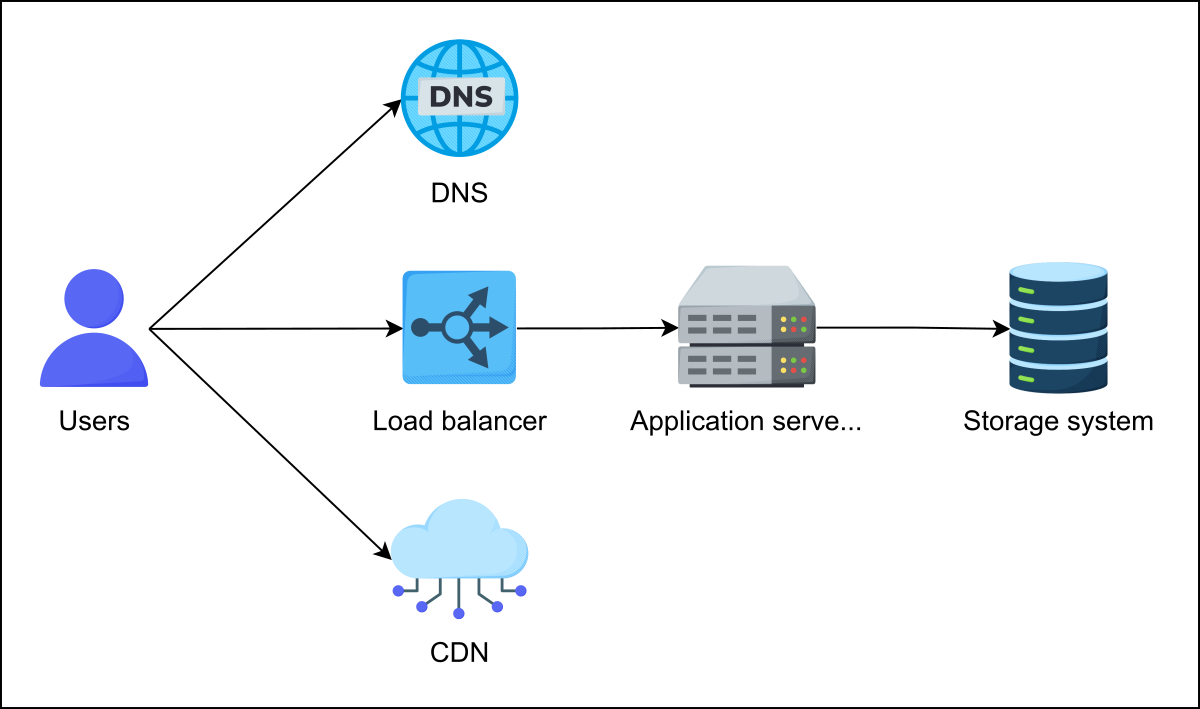
\includegraphics[width=0.5\textwidth]{Images/chapter_31/section_6194554750894080/6600608318881792.png}
 \caption{Twitter components}
\end{figure}

\begin{itemize}
\item
\protect\phantomsection\label{HcvVxQ2NWS-Do-RkjiLLr}
\textbf{Users} post Tweets delivered to the server through the load balancer. Then, the system stores it in persistent storage.
\item
\protect\phantomsection\label{4uY-JMxnfCA9JQQXk2Tpi}
\textbf{DNS} provides the specified IP address to the end user to start communication with the requested service.
\item
\protect\phantomsection\label{-OzVIfspS-WOBOs_pWbiZ}
\textbf{CDN} is situated near the users to provide requested data with low latency. When users search for a specified term or tag, the system first searches in the CDN proxy servers containing the most frequently requested content.
\item
\protect\phantomsection\label{xkLClnpk43h5T9XCmUCyL}
\textbf{Load balancer} chooses the operational application server based on traffic load on the available servers and the user requests.
\item
\protect\phantomsection\label{8fsOmkTh7GW_aaTNfI_tA}
\textbf{Storage system} represents the various types of storage (SQL-based and NoSQL-based) in the above illustration. We'll discuss significant storage systems later in this chapter.
\item
\protect\phantomsection\label{CLcbhAk19_jrh3K7znTix}
\textbf{Application servers} provide various services and have business logic to orchestrate between different components to meet our functional requirements.
\end{itemize}
\\
We have detailed chapters on \href{https://www.educative.io/courses/grokking-the-system-design-interview/introduction-to-domain-name-system-dns}{DNS}, \href{https://www.educative.io/courses/grokking-the-system-design-interview/system-design-the-content-delivery-network-cdn}{CDN}, specified storage systems (\href{https://www.educative.io/courses/grokking-the-system-design-interview/introduction-to-databases}{Databases}, \href{https://www.educative.io/courses/grokking-the-system-design-interview/system-design-the-key-value-store}{Key-value store}, \href{https://www.educative.io/courses/grokking-the-system-design-interview/system-design-a-blob-store}{Blob store}), and \href{https://www.educative.io/courses/grokking-the-system-design-interview/introduction-to-load-balancers}{Load balancers} in our building blocks section. We 'll focus on further details specific to the Twitter service in the coming lessons. Let
's first understand the service API.

\subsection{API design}\label{KYrzkUxDQM4BTxKIl8HQB}
\\
This section will focus on designing various APIs regarding the functionalities we are providing. We learn how users request various services through APIs. We 'll only concentrate on the significant parameters of the APIs that are relevant to our design. Although the front-end server can call another API or add more parameters in the API received from the end users to fulfill the given request, we consider all relevant arguments specified for the particular request in a single API. Let
's develop APIs for each of the following features:

\begin{itemize}
\item
\protect\phantomsection\label{fXs0N64gPoR1swlt7pUqX}
Post Tweet
\item
\protect\phantomsection\label{pVg-A-fU9qGuO0wqQZHKD}
Like or dislike Tweet
\item
\protect\phantomsection\label{1o_mj2ZuZi8yZ878UKFrU}
Reply to Tweet
\item
\protect\phantomsection\label{VHz5-ZSa2Df03iFY2KpN7}
Search Tweet
\item
\protect\phantomsection\label{A_j-5wB3rcDQUaaS3fknz}
View user or home timeline
\item
\protect\phantomsection\label{Ucasbi6wCXv833sg2cu44}
Follow or unfollow the account
\item
\protect\phantomsection\label{8tCXzgx2plpIc546k0NOf}
Retweet a Tweet
\end{itemize}

\subsubsection{Post Tweet}\label{TvBna7i06LnATcVFhf3w0}
\\
The POST method is used to send the Tweet to the server from the user through the \texttt{/postTweet} API.

\begin{lstlisting}[language=JavaScript]
postTweet(user_id, access_type, tweet_type, content, tweet_length, media_field, post_time, tweet_location, list_of_used_hashtags, list_of_tagged_people)
\end{lstlisting}

Let's discuss a few of the parameters:

\begin{table}[htbp]
\centering
\small
\adjustbox{max width=\textwidth}{
\begin{tabular}{|p{0.199\textwidth}|p{0.751\textwidth}|}
\hline
\textbf{Parameter} & \textbf{Description} \\
\hline
\hline
\texttt{user\_id} & It indicates the unique ID of the user who posted the Tweet.~ \\
\hline
\texttt{access\_type} & It tells us whether the Tweet is protected (that is, only visible to followers) or public. \\
\hline
\texttt{tweet\_type} & It indicates whether the Tweet is text-based, video-clip based, image(s)-based, or consisting of different types. \\
\hline
\texttt{content} & It specifies the Tweet's actual content (text). \\
\hline
\texttt{tweet\_length} & It represents the text length in the Tweet. In the case of video, it tells us the duration and size of a video.~ \\
\hline
\texttt{media\_field} & It specifies the type of media (image, video, GIF, and so on) delivered in each Tweet. \\
\hline
\end{tabular}
}
\end{table}

The rest of the parameters are self-explanatory.
\begin{quote}
\textbf{Note:} Twitter uses the \textbf{Snowflake} service to generate unique IDs for Tweets. We have a detailed chapter (\href{https://www.educative.io/courses/grokking-the-system-design-interview/system-design-sequencer}{Sequencer}) that explains this service.
\end{quote}

\begin{quote}
\textbf{Quiz:}
\textbf{Question 1:} At most, how many hashtags can a Tweet have?
\textbf{Answer:} The text limit is 280 characters in a Tweet. So, users can use the hashtag(s) such that text length (including plain text, any links, and hashtags) does not exceed the limit of 280 characters.
\textbf{Question 2:} What is the need for the `list\_of\_tagged\_people` in the `/postTweet`

API?
\textbf{Answer:} The system has to notify the people tagged in the Tweet.
\end{quote}

\subsubsection{Like or dislike Tweet}\label{F4S1nMvfqbU3d2uWR0_JA}
\\
The \texttt{/likeTweet} API is used when users like public Tweets.

\begin{lstlisting}[language=JavaScript]
likeTweet(user_id, tweet_id, tweeted_user_id, user_location)
\end{lstlisting}

\begin{table}[htbp]
\centering
\small
\adjustbox{max width=\textwidth}{
\begin{tabular}{|p{0.194\textwidth}|p{0.756\textwidth}|}
\hline
\textbf{Parameter} & \textbf{Description} \\
\hline
\hline
\texttt{user\_id} & It indicates the unique ID of the user who liked the Tweet. \\
\hline
\texttt{tweet\_id} & It indicates the Tweet\textquotesingle s unique ID. \\
\hline
\texttt{tweeted\_user\_id} & This is the unique ID of the user who posted the Tweet. \\
\hline
\texttt{user\_location} & It denotes the location of the user who liked the Tweet. \\
\hline
\end{tabular}
}
\end{table}

The parameters above are also used in the \texttt{/dislikeTweet} API when users dislike others' Tweets.

\subsubsection{Reply to Tweet}\label{HI0s26O48c3r-KM-QVgXk}
\\
The \texttt{/replyTweet} API is used when users reply to public Tweets.

\begin{lstlisting}[language=JavaScript]
replyTweet(user_id, tweet_id, tweeted_user_id, reply_type, reply_content, reply_length)
\end{lstlisting}

The reply\_type, reply\_content, and reply\_length parameters are the same as tweet\_type, \texttt{content}, and tweet\_length respectively.

\subsubsection{Search Tweet}\label{kR8eKGLLfsLy0UCogdOyG}
\\
When the user searches any keyword in the home timeline, the GET method is used. The following is the \texttt{/searchTweet} API:

\begin{lstlisting}[language=JavaScript]
searchTweet(user_id, search_term, max_result, exclude, media_field, expansions, sort_order, next_token, user_location)
\end{lstlisting}

Some new parameters introduced in this case are:

\begin{table}[htbp]
\centering
\small
\adjustbox{max width=\textwidth}{
\begin{tabular}{|p{0.194\textwidth}|p{0.756\textwidth}|}
\hline
\textbf{Parameter} & \textbf{Description} \\
\hline
\hline
\texttt{search\_term} & It is a string containing the search keyword or phrase. \\
\hline
\texttt{max\_result} & It is the number of Tweets returned per response page. By default, the Tweets per response is 10. \\
\hline
\texttt{exclude} & It specifies what to exclude from the returned Tweets, that is, replies and retweets. The maximum limit on returned Tweets is 3200, but when we exclude replies, the maximum limit is reduced to 800 Tweets. \\
\hline
\texttt{media\_field} & It specifies the media (image, video, GIF) delivered in each returned Tweet. \\
\hline
\texttt{expansions} & It enables us to request additional data objects in the returned Tweets, such as any mentioned user, referenced Tweet, attached media, attached places objects, and so on. \\
\hline
\texttt{sort\_order} & It specifies the order in which Tweets are returned. By default, it will return the most recent Tweets first. \\
\hline
\texttt{next\_token} & It is used to get the next page of results. For instance, if \texttt{max\_result} is set to 100 Tweets, and the result set contains 200 Tweets, then the value of \texttt{next\_token} is directly pulled from the response to request the next page containing the following 100 Tweets. The last result (page) will not have a \texttt{next\_token}. \\
\hline
\end{tabular}
}
\end{table}

\paragraph{Response}\label{P9pgX536ZvjbXiQr9PSrz}
\\
Let's look at a sample response in JSON format. The \textbf{id} is the user's unique ID who posted the Tweet and the \textbf{text} is the Tweet's content. The \textbf{result\_count} is the count of the returned Tweet, which we set in the max\_result in the request. Here, we're displaying the default fields only.

\begin{verbatim}
{
  "data": [
    {
      "id": "7300333948034441183",
      "text": "This is a most matched Tweet"
    },
    {
      "id": "6498431343154916376",
      "text": "This is next to most matched Tweet"
    },
                   : 
                   :
                   :
    {
      "id": "6427456107642019844",
      "text": "This is the last matched Tweet in the current page of the result.
    }
  ],
  "meta": {
    "newest_id": "7300333948034441183",
    "oldest_id": "6427456107642019844",
    "result_count": 10
  }
}
\end{verbatim}

\begin{quote}
\textbf{Note:} Twitter performs various types of searches. The following are two of them: * One search type returns the result of the last seven days, which all registered users usually use. * The other type returns all matching results on all Tweets ever posted (remind that service does not delete a posted Tweet). Indeed, matches can contain the first Tweet on Twitter. This search is usually used for academic research.
\end{quote}

\subsubsection{View home\_timeline}\label{KMmQfjAlz_0XCE4rtAhzb}
\\
The GET method is suitable when users view their home timelines through the /viewHome\_timeline API.

\begin{lstlisting}[language=JavaScript]
viewHome_timeline(user_id, tweets_count, max_result, exclude, next_token, user_location)
\end{lstlisting}

In the /viewHome\_timeline API, we'll exclude the user\_location to get the user timeline.
\\
The max\_result parameter determines the number of tweets a client application can show the user. The server sends the max\_result number of tweets in each response. Further , the server will also send a paginated list\_of\_followers to reduce the client latency.

\begin{quote}
\textbf{Quiz:}
\textbf{Question 1:} Which parameter in the `viewHome\_timeline` method is the most relevant when deciding which promoted ads (Tweets) to be returned in response?
\textbf{Answer:} The decision to send specified promoted ads is made on the

`user\_location` parameter. For example, the user belongs to the `NewYork` city, so most probably it gets promoted ads associated or originated in that region.
\end{quote}

\subsubsection{Follow the account}\label{iUcyFxPZiIsyufwJO7SQL}
\\
The \texttt{/followAccount} API is used when users follow someone's account on Twitter.

\begin{lstlisting}[language=JavaScript]
followAccount(account_id, followed_account_id)
\end{lstlisting}

\begin{table}[htbp]
\centering
\small
\adjustbox{max width=\textwidth}{
\begin{tabular}{|p{0.194\textwidth}|p{0.756\textwidth}|}
\hline
\textbf{Parameter} & \textbf{Description} \\
\hline
\hline
\texttt{account\_id} & It specifies the unique ID of a user who follows that account on Twitter. \\
\hline
\texttt{followed\_account\_id} & It indicates the unique ID of the account that the user follows. \\
\hline
\end{tabular}
}
\end{table}

The \texttt{/unfollowAccount} API will use the same parameters when a user unfollows someone's account on Twitter.

\subsubsection{Retweet a Tweet}\label{Zd0FdlFPA04LNlqpa3HeT}
\\
When a registered user Retweets (re-posts) someone's Tweet on Twitter, the following \texttt{/retweet} API is called:

\begin{lstlisting}[language=JavaScript]
retweet(user_id, tweet_id, retweet_user_id)
\end{lstlisting}

The same parameters will be required in the \texttt{/undoRetweet} API when users undo a Retweet of someone's Tweet.
\\
\textbf{Question:} It's New Year's Eve, and Twitter is expecting a huge surge in traffic. We have already provided a high-level design of the system with standard components like load balancers and CDN in place. Suggest additional enhancements or modifications required in the existing high-level design to ensure the platform can handle the traffic spike efficiently and maintain zero downtime.\\
\\


% End of section content